\documentclass{standalone}
\usepackage{tikz}
\usetikzlibrary{patterns, positioning}

\begin{document}
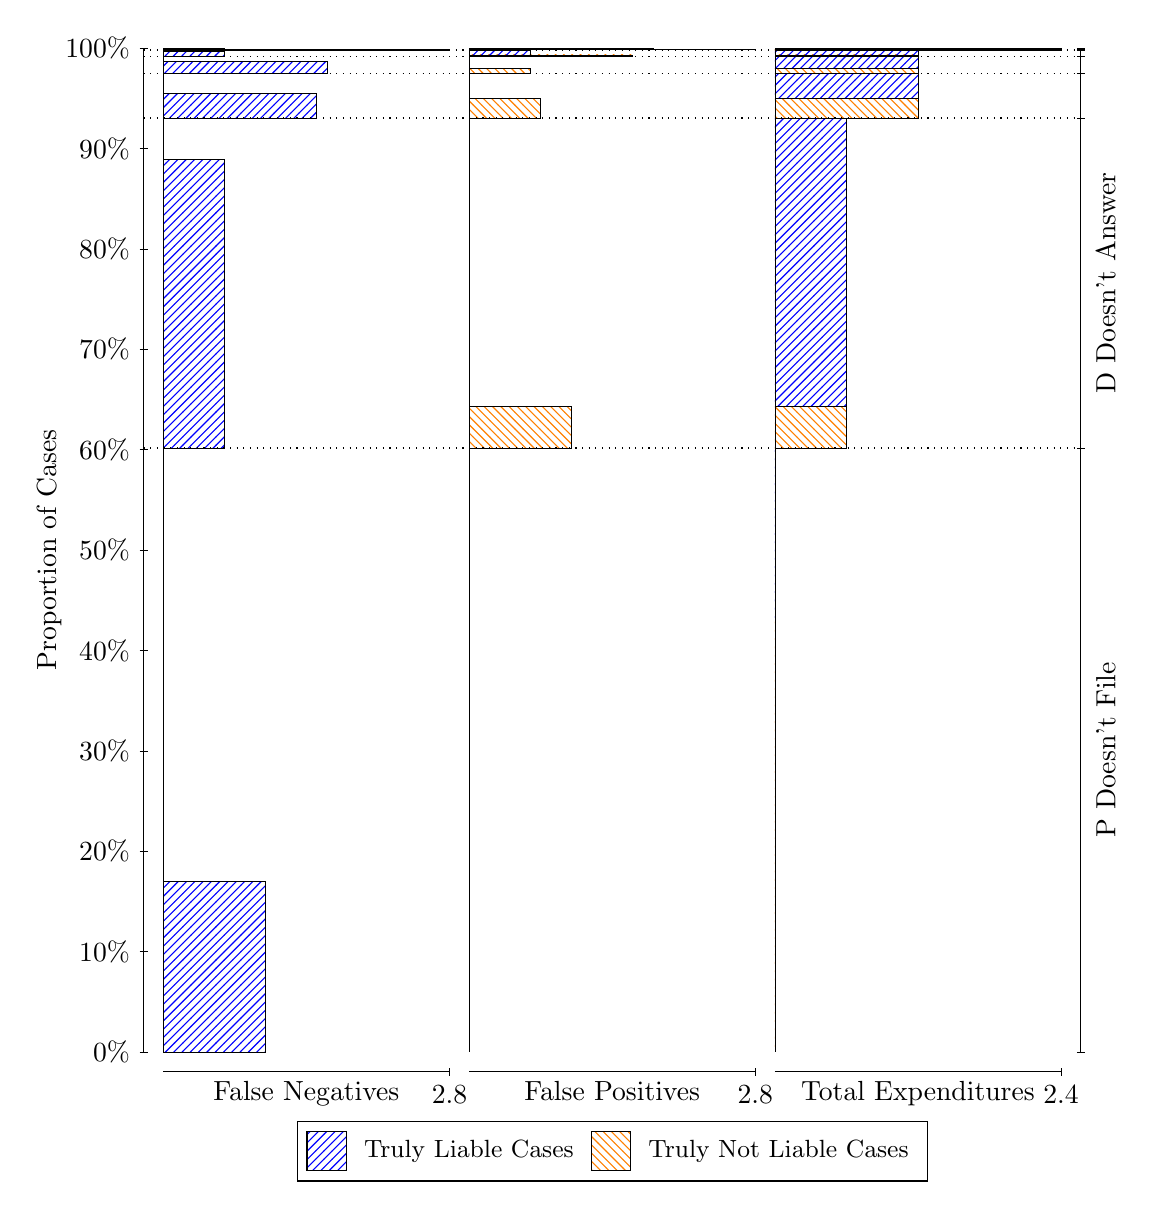
\begin{tikzpicture}
\draw[black, very thin] (1.5,1.75) -- (1.5,14.5);
\node[rotate=90, anchor=center] at (0.3, 8.125) {Proportion of Cases};
\draw[black, very thin] (1.45,1.75) -- (1.55,1.75);
\node[anchor=east] at (1.45, 1.75) {0\%};
\draw[black, very thin] (1.45,3.025) -- (1.55,3.025);
\node[anchor=east] at (1.45, 3.025) {10\%};
\draw[black, very thin] (1.45,4.3) -- (1.55,4.3);
\node[anchor=east] at (1.45, 4.3) {20\%};
\draw[black, very thin] (1.45,5.575) -- (1.55,5.575);
\node[anchor=east] at (1.45, 5.575) {30\%};
\draw[black, very thin] (1.45,6.85) -- (1.55,6.85);
\node[anchor=east] at (1.45, 6.85) {40\%};
\draw[black, very thin] (1.45,8.125) -- (1.55,8.125);
\node[anchor=east] at (1.45, 8.125) {50\%};
\draw[black, very thin] (1.45,9.4) -- (1.55,9.4);
\node[anchor=east] at (1.45, 9.4) {60\%};
\draw[black, very thin] (1.45,10.675) -- (1.55,10.675);
\node[anchor=east] at (1.45, 10.675) {70\%};
\draw[black, very thin] (1.45,11.95) -- (1.55,11.95);
\node[anchor=east] at (1.45, 11.95) {80\%};
\draw[black, very thin] (1.45,13.225) -- (1.55,13.225);
\node[anchor=east] at (1.45, 13.225) {90\%};
\draw[black, very thin] (1.45,14.5) -- (1.55,14.5);
\node[anchor=east] at (1.45, 14.5) {100\%};

\draw[black, very thin] (13.4,1.75) -- (13.4,14.5);
\draw[black, very thin] (13.35,1.75) -- (13.45,1.75);
\node[anchor=west] at (13.35, 1.75) {};
\draw[black, very thin] (13.35,9.4198) -- (13.45,9.4198);
\node[anchor=west] at (13.35, 9.4198) {};
\draw[black, very thin] (13.35,13.611) -- (13.45,13.611);
\node[anchor=west] at (13.35, 13.611) {};
\draw[black, very thin] (13.35,14.173) -- (13.45,14.173);
\node[anchor=west] at (13.35, 14.173) {};
\draw[black, very thin] (13.35,14.398) -- (13.45,14.398);
\node[anchor=west] at (13.35, 14.398) {};
\draw[black, very thin] (13.35,14.474) -- (13.45,14.474);
\node[anchor=west] at (13.35, 14.474) {};
\draw[black, very thin] (13.35,14.482) -- (13.45,14.482);
\node[anchor=west] at (13.35, 14.482) {};
\draw[black, very thin] (13.35,14.5) -- (13.45,14.5);
\node[anchor=west] at (13.35, 14.5) {};

\draw[black, very thin, pattern color=blue, pattern=north east lines] (1.75,1.75) rectangle (3.0476,3.9191);
\draw[black, very thin, pattern color=orange, pattern=north west lines] (1.75,3.9191) rectangle (1.75,9.4198);
\draw[black, very thin, pattern color=blue, pattern=north east lines] (1.75,9.4198) rectangle (2.5286,13.082);
\draw[black, very thin, pattern color=orange, pattern=north west lines] (1.75,13.082) rectangle (1.75,13.611);
\draw[black, very thin, pattern color=blue, pattern=north east lines] (1.75,13.611) rectangle (3.6964,13.919);
\draw[black, very thin, pattern color=orange, pattern=north west lines] (1.75,13.919) rectangle (1.75,14.173);
\draw[black, very thin, pattern color=blue, pattern=north east lines] (1.75,14.173) rectangle (3.8262,14.328);
\draw[black, very thin, pattern color=orange, pattern=north west lines] (1.75,14.328) rectangle (1.75,14.398);
\draw[black, very thin, pattern color=blue, pattern=north east lines] (1.75,14.398) rectangle (2.5286,14.459);
\draw[black, very thin, pattern color=orange, pattern=north west lines] (1.75,14.459) rectangle (1.75,14.474);
\draw[black, very thin, pattern color=blue, pattern=north east lines] (1.75,14.474) rectangle (5.3833,14.478);
\draw[black, very thin, pattern color=orange, pattern=north west lines] (1.75,14.478) rectangle (1.75,14.482);
\draw[black, very thin, pattern color=blue, pattern=north east lines] (1.75,14.482) rectangle (2.5286,14.496);
\draw[black, very thin, pattern color=orange, pattern=north west lines] (1.75,14.496) rectangle (1.75,14.5);
\draw[black, very thin, pattern color=orange, pattern=north west lines] (5.6333,1.75) rectangle (5.6333,7.2506);
\draw[black, very thin, pattern color=blue, pattern=north east lines] (5.6333,7.2506) rectangle (5.6333,9.4198);
\draw[black, very thin, pattern color=orange, pattern=north west lines] (5.6333,9.4198) rectangle (6.931,9.9484);
\draw[black, very thin, pattern color=blue, pattern=north east lines] (5.6333,9.9484) rectangle (5.6333,13.611);
\draw[black, very thin, pattern color=orange, pattern=north west lines] (5.6333,13.611) rectangle (6.5417,13.864);
\draw[black, very thin, pattern color=blue, pattern=north east lines] (5.6333,13.864) rectangle (5.6333,14.173);
\draw[black, very thin, pattern color=orange, pattern=north west lines] (5.6333,14.173) rectangle (6.4119,14.243);
\draw[black, very thin, pattern color=blue, pattern=north east lines] (5.6333,14.243) rectangle (5.6333,14.398);
\draw[black, very thin, pattern color=orange, pattern=north west lines] (5.6333,14.398) rectangle (7.7095,14.412);
\draw[black, very thin, pattern color=blue, pattern=north east lines] (5.6333,14.412) rectangle (6.4119,14.474);
\draw[black, very thin, pattern color=orange, pattern=north west lines] (5.6333,14.474) rectangle (6.4119,14.478);
\draw[black, very thin, pattern color=blue, pattern=north east lines] (5.6333,14.478) rectangle (5.6333,14.482);
\draw[black, very thin, pattern color=orange, pattern=north west lines] (5.6333,14.482) rectangle (9.2667,14.486);
\draw[black, very thin, pattern color=blue, pattern=north east lines] (5.6333,14.486) rectangle (7.969,14.5);
\draw[black, very thin, pattern color=orange, pattern=north west lines] (9.5167,1.75) rectangle (9.5167,7.2506);
\draw[black, very thin, pattern color=blue, pattern=north east lines] (9.5167,7.2506) rectangle (9.5167,9.4198);
\draw[black, very thin, pattern color=orange, pattern=north west lines] (9.5167,9.4198) rectangle (10.425,9.9484);
\draw[black, very thin, pattern color=blue, pattern=north east lines] (9.5167,9.9484) rectangle (10.425,13.611);
\draw[black, very thin, pattern color=orange, pattern=north west lines] (9.5167,13.611) rectangle (11.333,13.864);
\draw[black, very thin, pattern color=blue, pattern=north east lines] (9.5167,13.864) rectangle (11.333,14.173);
\draw[black, very thin, pattern color=orange, pattern=north west lines] (9.5167,14.173) rectangle (11.333,14.243);
\draw[black, very thin, pattern color=blue, pattern=north east lines] (9.5167,14.243) rectangle (11.333,14.398);
\draw[black, very thin, pattern color=orange, pattern=north west lines] (9.5167,14.398) rectangle (11.333,14.412);
\draw[black, very thin, pattern color=blue, pattern=north east lines] (9.5167,14.412) rectangle (11.333,14.474);
\draw[black, very thin, pattern color=orange, pattern=north west lines] (9.5167,14.474) rectangle (13.15,14.478);
\draw[black, very thin, pattern color=blue, pattern=north east lines] (9.5167,14.478) rectangle (13.15,14.482);
\draw[black, very thin, pattern color=orange, pattern=north west lines] (9.5167,14.482) rectangle (13.15,14.486);
\draw[black, very thin, pattern color=blue, pattern=north east lines] (9.5167,14.486) rectangle (13.15,14.5);
\draw[black, dotted] (1.5,9.4198) -- (13.4,9.4198);
\draw[black, dotted] (1.5,13.611) -- (13.4,13.611);
\draw[black, dotted] (1.5,14.173) -- (13.4,14.173);
\draw[black, dotted] (1.5,14.398) -- (13.4,14.398);
\draw[black, dotted] (1.5,14.474) -- (13.4,14.474);
\draw[black, dotted] (1.5,14.482) -- (13.4,14.482);
\draw[black, very thin] (1.75,1.5) -- (5.3833,1.5);
\node[anchor=north] at (3.5667, 1.5) {False Negatives};
\draw[black, very thin] (5.3833,1.45) -- (5.3833,1.55);
\node[anchor=north] at (5.3833, 1.45) {2.8};

\draw[black, very thin] (5.6333,1.5) -- (9.2667,1.5);
\node[anchor=north] at (7.45, 1.5) {False Positives};
\draw[black, very thin] (9.2667,1.45) -- (9.2667,1.55);
\node[anchor=north] at (9.2667, 1.45) {2.8};

\draw[black, very thin] (9.5167,1.5) -- (13.15,1.5);
\node[anchor=north] at (11.333, 1.5) {Total Expenditures};
\draw[black, very thin] (13.15,1.45) -- (13.15,1.55);
\node[anchor=north] at (13.15, 1.45) {2.4};

\node[black, centered, rotate=90] at (13.72, 5.5849) {P Doesn't File};
\node[black, centered, rotate=90] at (13.72, 11.515) {D Doesn't Answer};






\draw (7.449999999999999,1.5) node[draw=none] (baseCoordinate) {};
\begin{scope}[align=center]
        \matrix[scale=0.5, draw=black, below=0.5cm of baseCoordinate, nodes={draw}, column sep=0.1cm]{
            \node[rectangle, draw, minimum width=0.5cm, minimum height=0.5cm, pattern=north east lines, pattern color=blue] {}; &
            \node[draw=none, font=\small] (B) {Truly Liable Cases}; &
            \node[rectangle, draw, minimum width=0.5cm, minimum height=0.5cm, pattern=north west lines, pattern color=orange] {}; &
            \node[draw=none, font=\small] (B) {Truly Not Liable Cases}; \\
            };
\end{scope}

\end{tikzpicture}
\end{document}